Gestion de versions de grands textes 

Dans ce sujet, on s'intéresse à des textes de grande taille auxquels plusieurs auteurs apportent
des modifications au cours du temps. Ces textes peuvent par exemple être des programmes
informatiques développés par de multiples auteurs. Il est important de pouvoir efficacement
gérer les différentes versions de ces programmes au cours de leur développement et limiter le
stockage et la transmission d'informations redondantes. Nous allons pour cela nous intéresser à
une notion de \textit{différentiels} entre textes. 

\begin{defi}{Complexité}
La complexité, ou le temps d'exécution, d'une fonction $P$ est le nombre d'opérations élémentaires (addition, multiplication, affectation, test, etc ...) nécessaires à l'exécution
de $P$ dans le cas le pire. Lorsque la complexité dépend d'un ou plusieurs paramètres $\kappa_1$, ..., $\kappa_r$, on dit que $A$ a une complexité en $\mathcal{O}\left( f \left(\kappa_1, ..., \kappa_r  \right)\right)$ s'il existe une constante $C > 0$ telle que,
pour toutes les valeurs de $\kappa_1$, ..., $\kappa_r$ suffisamment grandes (c'est-à-dire plus grandes qu'un certain seuil), pour toute instance du problème de paramètres $\kappa_1$, ..., $\kappa_r$, la complexité est au plus
$C \cdot f \left(\kappa_1, ..., \kappa_r  \right)$.
\end{defi}

Lorsqu'il est demandé de donner la complexité d'un programme, le candidat devra justifier
cette dernière si elle ne se déduit pas directement de la lecture du code. 

\vspace{.5cm}

\textbf{Rappels concernant le langage}  \texttt{Python}
Ce sujet utilise les types Python listes et dictionnaires, mais seules les opérations mentionnées ci-dessous sont autorisées dans vos réponses. Quand une complexité est indiquée avec un symbole (*), cela signifie que nous faisons une hypothèse
simplificatrice sur sa complexité. La justification de cette simplification est hors-programme. 

Si \lstinline{l}, \lstinline{l1}, \lstinline{l2} désignent des listes en \lstinline{Python} : 
\begin{itemize}
\item  \lstinline{len(l)} renvoie la longueur de la liste \lstinline{l}, c'est-à-dire le nombre d'éléments qu'elle contient. Complexité en $\mathcal{O}(1)$;
\item  \lstinline{l1 == l2} teste l'égalité des listes \lstinline{l1} et \lstinline{l2}. Complexité en $\mathcal{O}(n)$ avec $n$ le minimum de \lstinline{len(l1)} et \lstinline{len(l2)};
\item  \lstinline{l[i]} désigne le \lstinline{i}-ème élément de la liste \lstinline{l}, où l'indice \lstinline{i} est compris entre \lstinline{0} et \lstinline{len(l)-1}. Complexité en $\mathcal{O}(1)$;
\item  \lstinline{l[i: j]} construit la sous-liste \lstinline{[l[i] , ... , l[j-1]]}. Complexité en $\mathcal{O}(j-i)$. L'usage des variantes \lstinline{l[i:]} à la place de \lstinline{l[i:len(l)]}, et de \lstinline{l[:j]} à la place de \lstinline{l[0:j]} est aussi autorisé. 
\item \lstinline{l.append(e)} modifie la liste \lstinline{l} en lui ajoutant l'élément e en dernière position. Complexité en $\mathcal{O}(1)$ (*).
\item \lstinline{l.pop()} renvoie le dernier élément de la liste \lstinline{l} (supposée non vide) et supprime l'occurrence de cet élément en dernière position dans la liste. Complexité en $\mathcal{O}(1)$ (*).
\end{itemize} 
On pourra aussi utiliser la fonction \lstinline{range} pour réaliser des itérations.

\vspace{.5cm}

Si \lstinline{d} est un dictionnaire Python :
\begin{itemize}
\item \{\lstinline{key_1: v_1, ..., key_n: v_n}\} crée un nouveau dictionnaire en associant chaque valeur
\lstinline{v_i} à une clé \lstinline{key_i}. Complexité en $\mathcal{O}(n)$ (*).
\item \lstinline{d[key]} renvoie la valeur associée à la clé \lstinline{key} dans \lstinline{d} et lève une erreur si la clé key n'est
pas présente. Complexité en $\mathcal{O}(1)$ (*).
\item \lstinline{d[key] = v} modifie \lstinline{d} pour associer la valeur \lstinline{v} à la clé \lstinline{key}, même si la clé \lstinline{key} n'est pas
présente dans \lstinline{d} initialement. Complexité en $\mathcal{O}(1)$ (*).
\item \lstinline{key} in \lstinline{d} teste si la clé \lstinline{key} est présente dans \lstinline{d}. Complexité en $\mathcal{O}(1)$ (*).
\end{itemize}

Sauf mention contraire, les fonctions à écrire ne doivent pas modifier leurs entrées.

La structure de données texte. Dans ce sujet, on appelle texte une liste de caractères. Par
exemple, \lstinline{['b', 'i', 'n', 'g', 'o']} est un texte de longueur 5.


\section*{Partie I : Différentiels par positions fixes}
Dans cette partie, nous traitons le problème avec une hypothèse simplificatrice : les textes
comparés ont toujours la même taille.

%Question 1. 
\question{Sans utiliser le test \lstinline{==} sur les listes, écrire une fonction 
\lstinline{textes_égaux(texte1,texte2)} qui teste si deux textes sont égaux. Donner la complexité de cette fonction.}
\ifprof
\begin{corrige}~\\ 
\vspace{-.5cm}
\begin{lstlisting}
def textes_égaux(texte1, texte2) :
    for i in range(len(texte1)) :
        if texte1[i] != texte2[i] :
            return False
    return True
\end{lstlisting}
En notant $n$ la longueur de \lstinline{texte1} et \lstinline{texte2}, cette fonction a une complexite $\mathcal{O}(n)$.
\end{corrige}
\else

\fi
\begin{exemple}~\\ 
\vspace{-.5cm}
\begin{lstlisting}
>>> textes_égaux(['v', 'i', 's', 'a'], ['v', 'a', 'i', 's'])
False
>>> textes_égaux(['v', 'i', 's', 'a'], ['v', 'i', 's', 'a'])
True
\end{lstlisting}
\end{exemple}


Dans la suite de ce sujet, on pourra utiliser \lstinline{==} sur les listes plutôt que cette fonction.

Si deux textes ne sont pas égaux mais ont la même longueur $n$, on souhaite compter le nombre
de positions qui diffèrent, c'est à dire déterminer combien il existe de positions $i$ ($0\leq i < n$)
telles que les caractères en position $i$ sont différents dans les deux textes.

\question{Écrire une fonction \lstinline{distance(texte1, texte2)} qui calcule cette quantité. On
supposera que les deux textes ont le même nombre de caractères. Donner la complexité de cette
fonction.}
\ifprof
\begin{corrige}~\\ 
\vspace{-.5cm}
\begin{lstlisting}
def distance(texte1, texte2) :
    cpt = 0
    for i in range(len(texte1)) : 
        if texte1[i] != texte2[i] :
            cpt = cpt + 1
    return cpt
\end{lstlisting}
En notant $n$ la longueur de \lstinline{texte1} et \lstinline{texte2}, cette fonction a une complexite $\mathcal{O}(n)$.
\end{corrige}
\else
\fi

\begin{exemple}~\\ 
\vspace{-.5cm}
\begin{lstlisting}
>>> distance(['v', 'i', 's', 'a'], ['v', 'a', 'i', 's'])
3
>>> distance(['a', 'v', 'i', 's'], ['v', 'i', 's', 'a'])
4
\end{lstlisting}
\end{exemple}

%Question 3. 
\question{En vous aidant d'un dictionnaire dont les clés sont des caractères, écrire une fonction \lstinline{aucun_caractère_commun(texte1, texte2)} qui renvoie \lstinline{True} si et seulement si l'ensemble
des caractères qui apparaissent dans \lstinline{texte1} est disjoint de l'ensemble des caractères qui apparaissent dans \lstinline{texte2}. Les deux textes peuvent avoir ici des longueurs différentes. Cette fonction devra avoir une complexité $\mathcal{O}\left(\text{len(texte1)} + \text{len(texte2)}\right)$.}
\ifprof
\begin{corrige}~\\ 
\vspace{-.5cm}
\begin{lstlisting}
def aucun_caractère_commun(texte1, texte2) :
    # Création d'un dictionnaire listant les caractères
\end{lstlisting}
\end{corrige}
\else
\fi


\begin{exemple}~\\ 
\vspace{-.5cm}
\begin{lstlisting}
>>> aucun_caractère_commun(['a', 'v', 'i', 's'], ['v', 'i', 's', 'a'])
False
>>> aucun_caractère_commun(['a', 'v', 'i', 's'], ['u', 'r', 'n', 'e'])
True
\end{lstlisting}
\end{exemple}

Nous introduisons maintenant une structure de données spécifique pour représenter un différentiel par positions fixes entre deux textes.
La Figure \ref{fig:01} présente un exemple de couple de textes (texte1, texte2) qui diffèrent sur 4
tranches (représentées par des zones grisées sur la figure). En dehors des tranches, les textes sont
égaux.

\begin{figure}[H]
\centering
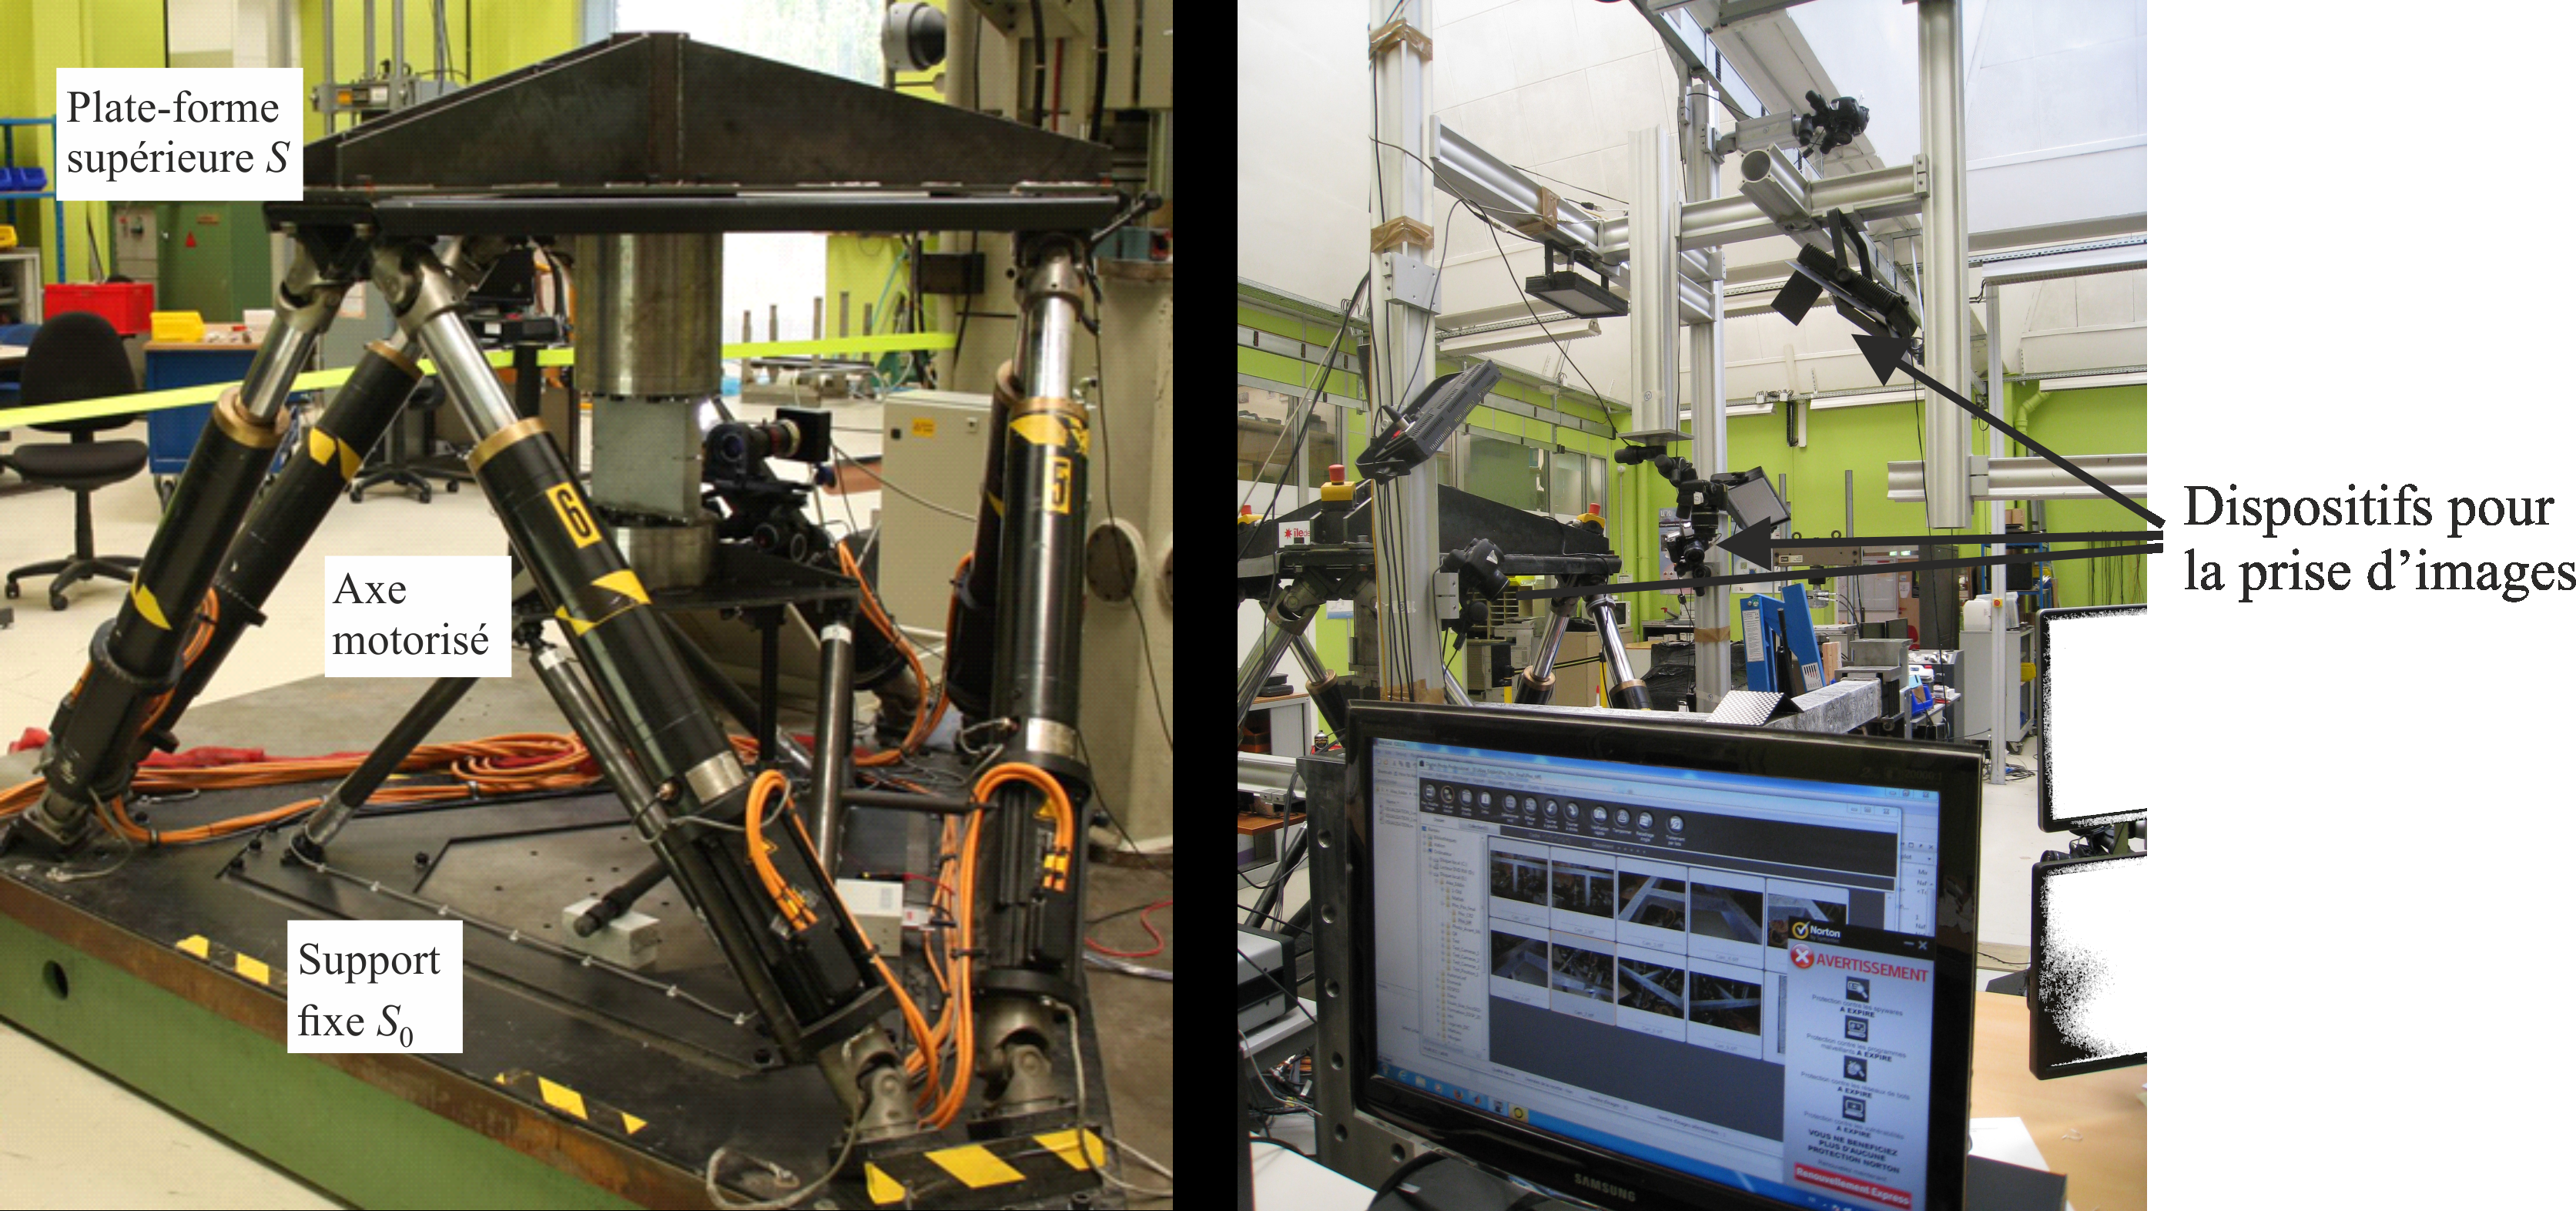
\includegraphics[width=.8\linewidth]{fig_01}
\caption{Exemple de couple (texte1, texte2) dont on veut calculer le différentiel (sur des
positions fixes) \label{fig:01}}
\end{figure}

\begin{defi}{La structure de données tranche.} Une tranche est un dictionnaire avec trois clés \lstinline{'début'},
\lstinline{'avant'} et \lstinline{'après'}. La valeur associée à la clé \lstinline{'début'} est le premier indice de la tranche, les
extes associés aux clés \lstinline{'avant'} et \lstinline{'après'} représentent les textes (de même longueur) de la tranche avant et après modification. Dans la suite de cette partie, on s'appuiera sur les fonctions
suivantes pour manipuler cette structure.
\end{defi}

\begin{lstlisting}
def tranche(arg_début, arg_avant, arg_après):
    return {'début': arg_début, 'avant': arg_avant, 'après': arg_après}

def début(tr):
    return tr['début']

def après(tr):
    return tr['après']

def avant(tr):
    return tr['avant']

def fin(tr):
    return début(tr) + len(après(tr))
\end{lstlisting}

Nous ne fournissons pas de fonction pour modifier une tranche car nous souhaitons traiter
cette structure de données comme une structure immuable\footnote{On rappelle qu'une structure immuable est une structure qui n'est jamais modifiée. C'est par exemple le
cas des chaînes et des tuples en Python.}.
On peut représenter le différentiel de la Figure \ref{fig:01}, par la liste suivante :

\begin{lstlisting}
[
tranche(3, ['g', 'r', 'a', 'n', 'd'], ['p', 'e', 't', 'i', 't']),
tranche(11, ['â', 't', 'e', 'a', 'u'], ['i', 'e', 'n', ' ', 'a']),
tranche(17, ['f'], ['s']),
tranche(19, ['r', 't'], ['i', 'f'])
]
\end{lstlisting}

\begin{defi}{La structure de données \textit{différentiel}}. Un \textit{différentiel} est une liste (potentiellement vide)
de tranches \lstinline{[tr1, ..., trk]} représentant des modifications touchant des zones distinctes d'un
texte, telle que :
\begin{itemize}
\item \lstinline{début(tr1)} $<$ \lstinline{fin(tr1)} $<$ ... $<$ \lstinline{début(trk) < fin(trk)};
\item pour tout $j \in [1, k]$, pour tout $i \in$ \lstinline{[0, len(avant(trj ))-1]}, \lstinline{avant(trj )[i]} $\neq$ \lstinline{après(trj)[i]}.  
\end{itemize}
\end{defi}

\begin{prop}{Existence et unicité d'un différentiel par positions fixes.} Pour deux textes \lstinline{texte1} et
\lstinline{texte2} de même longueur $n$, il existe un unique différentiel \lstinline{[tr1, ..., trk]} tel que :
\begin{itemize}
\item si $k > 0$, alors $0 \leq$ \lstinline{début(tr1)} et \lstinline{fin(trk)} $\leq n $;
\item pour tout $j \in [1, k]$, \lstinline{texte1[début(trj ) : fin(trj )] = avant(trj)};
\item pour tout $j \in [1, k]$, \lstinline{texte2[début(trj ) : fin(trj )] = après(trj)};
\item pour tout $i \in [0, n-1]$, si $i \notin \cup_{1\leq j \leq k}$
\lstinline{[début(trj), fin(trj )-1]}, alors \lstinline{texte1[i] = texte2[i]}.
\end{itemize}
\end{prop}

Cet unique différentiel est appelé le \textit{différentiel} de \lstinline{texte2} vis-à-vis de \lstinline{texte1}.

Toutes les propriétés précédentes sur les différentiels assurent les propriétés intuitives suivantes :
\begin{itemize}
\item les tranches sont présentées par indices de début croissants, sans se chevaucher, ni se toucher ;
\item chaque tranche \lstinline{tr} couvre un intervalle de positions \lstinline{[début(tr), fin(tr)-1]} sur lequel 
\lstinline{texte1} et \lstinline{texte2} diffèrent à chaque position, et dont les sous-textes sur ces intervalles
correspondent à \lstinline{avant(tr)} pour \lstinline{texte1} et \lstinline{après(tr)} pour \lstinline{texte2}.
\end{itemize}


%Question 4. 
\question{Écrire une fonction \lstinline{différentiel(texte1, texte2)} qui calcule le différentiel du
texte \lstinline{texte2} vis-à-vis du texte \lstinline{texte1}, supposés de même longueur. La complexité attendue est $\mathcal{O}$\lstinline{(len(texte1))}. Justifier cette complexité.}
\ifprof
\begin{corrige}~\\ 
\vspace{-.5cm}
\begin{lstlisting}
#
\end{lstlisting}
\end{corrige}
\else
\fi


%Question 5. 
\question{Écrire une fonction \lstinline{applique(texte1, diff)} qui, étant donné un texte \lstinline{texte1} et
un différentiel \lstinline{diff}, renvoie un texte \lstinline{texte2} tel que \lstinline{diff} soit le différentiel de \lstinline{texte2} vis-à-vis
de \lstinline{texte1}. On supposera que le différentiel diff contient des tranches cohérentes avec la taille
et le contenu du texte \lstinline{texte1}. Donner et justifier la complexité.}
\ifprof
\begin{corrige}~\\ 
\vspace{-.5cm}
\begin{lstlisting}
#
\end{lstlisting}
\end{corrige}
\else
\fi



Pour reconstruire l'ancienne version d'un texte à partir d'un différentiel, nous allons nous
appuyer sur la notion de différentiel inversé.

%Question 6. 
\question{Écrire une fonction \lstinline{inverse(diff)} telle que pour tous textes \lstinline{texte1}, \lstinline{texte2}
de même longueur, si \lstinline{diff} désigne \lstinline{différentiel(texte1, texte2)}, alors \lstinline{applique(texte2,
inverse(diff)) = texte1} et \lstinline{inverse(inverse(diff)) = diff}. Donner sa complexité.}
\ifprof
\begin{corrige}~\\ 
\vspace{-.5cm}
\begin{lstlisting}
#
\end{lstlisting}
\end{corrige}
\else
\fi


\textbf{La structure de données \textit{texte versionné}}. Nous représentons un texte versionné par un
dictionnaire contenant la version courante du texte, comme valeur associée à la clé \lstinline{'courant'},
et l'historique des différentiels qui ont mené jusqu'à cette version dans une pile\footnote{Une pile est ici implémentée par une liste Python.} de différentiels
associée à la clé \lstinline{historique}. Dans la suite de cette partie, on s'appuiera sur les fonctions suivantes
pour manipuler cette structure.

\begin{lstlisting}
def versionne(texte):
    return {'courant' : texte, 'historique' : [] }

def courant(texte_versionné):
    return texte_versionné['courant']

def remplace_courant(texte_versionné, texte):
    texte_versionné['courant'] = texte

def historique(texte_versionné):
    return texte_versionné['historique']
\end{lstlisting}


Contrairement à la structure immuable de tranche, nous nous autorisons cette fois à modifier la structure de texte versionné, en particulier la pile qu'elle contient via les opérations
\lstinline{historique(texte_versionné).append(diff)} et \lstinline{historique(texte_versionné).pop()}.


%Question 7. 
\question{Écrire les fonctions \lstinline{modifie(texte_versionné, texte)} et
\lstinline{annule(texte_versionné)} qui assurent les deux opérations de base attendues sur un
texte versionné \lstinline{texte_versionné}. La fonction \lstinline{modifie(texte_versionné, texte)} modifie
\lstinline{texte_versionné} pour lui ajouter une nouvelle version correspondant au texte \lstinline{texte}, en
supposant qu'il a la même longueur $n$ que le texte courant. La taille de l'historique augmente alors de 1. La fonction ne renvoie rien. La fonction \lstinline{annule(texte_versionné)} modifie
\lstinline{texte_versionné} en annulant l'effet de la dernière modification effectuée et renvoie la nouvelle
valeur courante du texte. La taille de l'historique diminue alors de 1. On suppose que la pile des
différentiels n'est pas vide lors de cet appel. Donnez les complexités de ces deux fonctions.}
\ifprof
\begin{corrige}~\\ 
\vspace{-.5cm}
\begin{lstlisting}
#
\end{lstlisting}
\end{corrige}
\else
\fi


\begin{exemple}~\\ 
\vspace{-.5cm}
\begin{lstlisting}
>>> texte_versionné = versionne(['a', 'v', 'i', 's'])
>>> modifie(texte_versionné, ['v', 'i', 's', 'a'])
>>> modifie(texte_versionné, ['v', 'i', 't', 'a'])
>>> modifie(texte_versionné, ['l', 'i', 's', 'a'])
>>> assert courant(texte_versionné) == ['l', 'i', 's', 'a']
>>> assert historique(texte_versionné) == [
    différentiel(['a', 'v', 'i', 's'], ['v', 'i', 's', 'a']),
    différentiel(['v', 'i', 's', 'a'], ['v', 'i', 't', 'a']),
    différentiel(['v', 'i', 't', 'a'], ['l', 'i', 's', 'a'])
]
>>> annule(texte_versionné)
['v', 'i', 't', 'a'])
>>> annule(texte_versionné)
['v', 'i', 's', 'a'])
>>> annule(texte_versionné)
['a', 'v', 'i', 's']
\end{lstlisting}
\end{exemple}

\section*{Partie II : Différentiels sur des positions variables}

Dans cette partie, nous nous intéressons à des différentiels de textes dont les longueurs ne
sont plus forcément égales. Nous adaptons pour cela la définition de tranche et de différentiel. La
Figure \ref{fig:02} présente un exemple de couple \lstinline{(texte1, texte2)} dont on va représenter le différentiel
par une liste de tranches (représentées par des zones grisées sur la figure). Cette fois, les tranches
désignent des portions de textes qui ne sont pas nécessairement de la même longueur, ni alignées.

\begin{figure}[H]
\centering
\includegraphics[width=.8\linewidth]{fig_02}
\caption{Exemple de couple (\lstinline{texte1}, \lstinline{texte2}) dont on veut calculer le différentiel sur des
positions variables \label{fig:02}}
\end{figure}


Nouvelle structure de données tranche. Un différentiel d'un texte \lstinline{texte2} vis-à-vis d'un
texte \lstinline{texte1} est toujours une liste de tranches mais chaque tranche comporte maintenant 4 clés :
\begin{itemize}
\item la clé \lstinline{'début_avant'} représente la position $i$ d'un sous-texte avant qui a été supprimé de
\lstinline{texte1} ;
\item la clé \lstinline{'avant'} est associée au texte avant ;
\item la clé \lstinline{'début_après'} représente la position dans \lstinline{texte2} d'un sous-texte après, qui a été
ajouté à la place du sous-texte avant en position $i$ dans \lstinline{texte1};
\item la clé \lstinline{'après'} est associée au texte après.
\end{itemize}
Dans la suite de cette partie, on s'appuiera sur les fonctions suivantes pour manipuler cette
structure.


\begin{lstlisting}
def tranche(arg_début_avant, arg_avant, arg_début_après, arg_après):
    return {'début_avant': arg_début_avant,
            'avant': arg_avant,
            'début_après': arg_début_après,
            'après': arg_après}

def début_avant(tr):
    return tr['début_avant']

def début_après(tr):
    return tr['début_après']

def après(tr):
    return tr['après']

def avant(tr):
    return tr['avant']

def fin_avant(tr):
    return début_avant(tr) + len(avant(tr))

def fin_après(tr):
    return début_après(tr) + len(après(tr))
\end{lstlisting}


\begin{defi}{Nouvelle structure de données \textit{différentiel}.} Un différentiel est une liste (potentiellement
vide) de tranches \lstinline{[tr1, ..., trk]} telle que :
\begin{itemize}
\item \lstinline{début_avant(tr1)} $\leq$ \lstinline{fin_avant(tr1)} $<$...$<$ \lstinline{début_avant(trk)} $\leq$ \lstinline{fin_avant(trk)};
\item \lstinline{début_après(tr1)} $\leq$ \lstinline{fin_après(tr1)} $<$ ... $<$ \lstinline{début_après(trk)} $\leq$ \lstinline{fin_après(trk)};
\item pour tout $j \in [1, k]$, \lstinline{aucun;_caractère_commun(avant(trj)}, \lstinline{après(trj )) = True}
\item pour tout $j \in [1, k]$, \lstinline{len(avant(trj)) > 0} ou \lstinline{len(après(trj)) > 0}.
\end{itemize}
\end{defi}

\begin{prop}{Notion de différentiel valide vis-à-vis de deux textes.} Pour deux textes \lstinline{texte1} et \lstinline{texte2}
de même longueur n, un différentiel valide de \lstinline{texte2} vis-à-vis de texte1 est une liste 
\lstinline{diff = [tr1, ..., trk]} de tranches telle que :
\begin{itemize}
\item si $k > 0$, alors $0 \leq$ \lstinline{début_avant(tr1)} et \lstinline{fin_avant(tr)} $\leq$ \lstinline{len(texte1)}
\item si $k > 0$, alors $0 \leq$ \lstinline{début_après(tr1)} et \lstinline{fin_après(trk)} $\leq$ \lstinline{len(texte2)}
\item pour tout $j \in [1, k]$, \lstinline{texte1[début_avant(trj)} : \lstinline{fin_avant(trj )] = avant(trj)};
\item pour tout $j \in [1, k]$, \lstinline{texte2[début_après(trj)} : \lstinline{fin_après(trj )] = aprèes(trj)};
\item pour tout $j \in [1, k-1]$,  les sous-textes \lstinline{texte1[fin_avant(trj)} : \lstinline{début_avant(trj+1)]} et
\lstinline{texte2[fin_après(trj)} : \lstinline{début_après(trj+1)]} sont égaux;
\item si $k = 0$ alors les textes \lstinline{texte1} et \lstinline{texte2} sont égaux;
\item si $k > 0$ alors \lstinline{texte1[0 : début_avant(tr1)] = texte2[0 : début_après(tr1)]} et
\lstinline{texte1[fin_avant(trk) : len(texte1)] = texte2[fin_après(trk) : len(texte2)]}
\end{itemize}
\end{prop}

On peut représenter le différentiel de la Figure \ref{fig:02}, par la liste suivante :
\begin{lstlisting}
[
tranche( 2, [], 2, [' ', 'b', 'o', 'n']),
tranche( 5, ['â', 't'], 9, ['i']),
tranche( 8, [], 11, ['n', ' ']),
tranche( 9, ['u'], 14, []),
tranche(11, ['f'], 15, ['s']),
tranche(13, ['r', 't'], 17, ['i', 'f'])
]
\end{lstlisting}

On admet que, comme dans la partie précédente, on peut écrire des fonctions \lstinline{applique}
et \lstinline{inverse} satisfaisant les mêmes propriétés que précédemment sur cette nouvelle notion de
différentiel. On définit le poids d'un différentiel comme la somme des longueurs des sous-textes
\lstinline{avant(tr)} et \lstinline{après(tr)} pour toutes les tranches \lstinline{tr} qui le composent.

%Question 8. 
\question{Écrire une fonction \lstinline{poids(diff)} qui calcule le poids d'un différentiel \lstinline{diff}. Donner
sa complexité.}
\ifprof
\begin{corrige}~\\ 
\vspace{-.5cm}
\begin{lstlisting}
#
\end{lstlisting}
\end{corrige}
\else
\fi


\begin{exemple}~\\ 
\vspace{-.5cm}
\begin{lstlisting}
>>> poids([tranche(0, ['b'], 0, ['t', 'r', 'o', 't', 't']),
            tranche(2, ['c', 'y', 'c', 'l'], 6, ['n'])])
11
\end{lstlisting}
\end{exemple}

On s'intéresse à la \textit{distance d'édition\footnote{Cette distance est communément appelée distance de Levenshtein.}} entre deux textes. Dans ce sujet, on définit cette
distance comme le nombre minimal de suppressions et d'insertions de caractères pour passer
d'un texte à un autre. On peut facilement se convaincre que cette distance coïncide avec le poids
minimal possible pour un différentiel entre les deux textes.

Nous allons calculer cette distance par programmation dynamique. Pour deux textes \lstinline{texte1}
et \lstinline{texte2} fixés, et pour $0 \leq i \leq $ \lstinline{len(texte1)} et $0 \leq j \leq$ \lstinline{len(texte2)}, on note $M[i][j]$ la distance
d'édition pour passer de \lstinline{texte1[0 : i]} à \lstinline{texte2[0 : j]}. La matrice\footnote{Dans ce sujet, nous représenterons ces matrices par des listes de listes d'entiers.} $M$ est appelée matrice de
distance d'édition entre \lstinline{texte1} et \lstinline{texte2}.

La Figure \ref{fig:03} présente la matrice M pour \lstinline{texte1 = ['A','B','C','D','C','E','F']} et
\lstinline{texte2 = ['U','A','B','C','C','X','Y','Z']}.

% Question 9. 
\question{Donnez une équation de récurrence qui exprime $M[i + 1][j + 1]$ en fonction de
$M[i][j]$, $M[i][j + 1]$, $M[i + 1][j]$, \lstinline{texte1[i]} et \lstinline{texte2[j]}, pour $0 \leq i < $\lstinline{len(texte1)} et $0 \leq j <$\lstinline{len(texte2)}. Justifier brièvement la validité de cette équation, sans rédiger une preuve complète.}
\ifprof
\begin{corrige}~\\ 
\vspace{-.5cm}
\begin{lstlisting}
#
\end{lstlisting}
\end{corrige}
\else
\fi

%Question 10. 
\question{Écrire une fonction \lstinline{levenshtein(texte1, texte2)} de complexité polynomiale
qui renvoie la matrice $M$. Préciser sa complexité.}
\ifprof
\begin{corrige}~\\ 
\vspace{-.5cm}
\begin{lstlisting}
#
\end{lstlisting}
\end{corrige}
\else
\fi

On utilisera l'instruction \lstinline{M = [[ 0 for j in range(m)] for i in range(n)]} pour initialiser une matrice \lstinline{M} de \lstinline{n} lignes et \lstinline{m} colonnes avec des zéros.

\begin{figure}[H]
\centering
\includegraphics[width=.6\linewidth]{fig_03}
\caption{Exemple de matrice de distances d'édition \label{fig:03}}
\end{figure}


%Question 11. 
\question{Écrire une fonction \lstinline{différentiel(texte1, texte2, M)} qui calcule un différentiel du texte \lstinline{texte2} vis-à-vis du texte \lstinline{texte1}, en s'aidant de la matrice de distance $M$ donnée
par \lstinline{levenshtein(texte1, texte2)}. Le différentiel renvoyé doit être de poids minimal. La fonction devra avoir une complexité $\mathcal{O}$(\lstinline{len(texte1) + len(texte2)}). Justifier cette complexité et
expliquer brièvement pourquoi le différentiel calculé satisfait les propriétés attendues par un
différentiel. On pourra s'aider de la Figure \ref{fig:03} pour comprendre quel parcours suivre dans la
matrice \lstinline{M}.}
\ifprof
\begin{corrige}~\\ 
\vspace{-.5cm}
\begin{lstlisting}
#
\end{lstlisting}
\end{corrige}
\else
\fi


Si on se place dans un scénario de travail collaboratif où deux auteurs différents modifient en
parallèle le même texte \lstinline{texte}, il est nécessaire de pouvoir fusionner leur travail. Nous notons
\lstinline{texte1} le nouveau texte obtenu après le travail du premier auteur sur \lstinline{texte} et \lstinline{diff1} le différentiel correspondant. De même, nous notons \lstinline{texte2} le texte obtenu après le travail du deuxième
auteur sur le même texte \lstinline{texte}, et \lstinline{diff2} le différentiel correspondant.

\begin{exemple}~\\ 
\vspace{-.5cm}
\begin{lstlisting}
>>> texte =
['l', 'e', ' ', 'c', 'h', 'a', 't', ' ', 'a', ' ', 's', 'o', 'i', 'f']
>>> texte1 =
['l', 'e', ' ', 'c', 'h', 'a', 't', ' ', 'a', ' ', 't', 'r', 'è', 's',
' ', 's', 'o', 'i', 'f']
>>> texte2 =
['l', 'e', ' ', 'c', 'h', 'i', 'e', 'n', ' ', 'a', ' ', 's', 'o', 'i', 'f']
>>> diff1 = différentiel(texte, texte1, levenshtein(texte, texte1))
>>> assert diff1 == [tranche(9, [], 9, [' ', 't', 'r', 'è', 's'])]
>>> diff2 = différentiel(texte, texte2, levenshtein(texte, texte2))
>>> assert diff2 == [tranche(5, ['a', 't'], 5, ['i', 'e', 'n'])]
\end{lstlisting}
\end{exemple}

Pour fusionner le travail des deux auteurs, on apporte des modifications à \lstinline{diff2} de façon
à ce que le texte final, qui inclut les modifications des deux auteurs, soit exprimable comme
l'application du différentiel \lstinline{diff1}, puis de la nouvelle version de \lstinline{diff2} sur le texte initial. Dans
l'exemple précèdent, le texte final attendu est : 
\lstinline{['l', 'e', ' ', 'c', 'h', 'i', 'e', 'n',' ', 'a', ' ', 't', 'r', 'è', 's', ' ', 's', 'o', 'i', 'f']}.


Nous allons être prudents en nous assurant au préalable que les modifications apportées ne
concernent pas les même zones du texte initial.

%Question 12. 
\question{Écrire une fonction \lstinline{conflit(diff1, diff2)} qui prend en argument deux différentiels \lstinline{diff1} et \lstinline{diff2} et renvoie \lstinline{True} si et seulement s'il existe une tranche \lstinline{tr1} dans \lstinline{diff1} et
une tranche \lstinline{tr2} dans \lstinline{diff2} telles que
\lstinline{[début_avant(tr1), fin_avant(tr1)] \ début_avant(tr2), fin_avant(tr2)]} $\neq$  \lstinline{0}. Cette fonction devra avoir une complexité $\mathcal{O}$(\lstinline{len(diff1) + len(diff2)}) que l'on justifiera.}

\ifprof
\begin{corrige}~\\ 
\vspace{-.5cm}
\begin{lstlisting}
#
\end{lstlisting}
\end{corrige}
\else
\fi


%Question 13. 
\question{Écrire une fonction \lstinline{fusionne(diff1, diff2)} qui renvoie un nouveau différentiel
représentant la mise à jour de \lstinline{diff2}. Il est attendu que \lstinline{poids(fusionne(diff1, diff2)) = poids(diff2)}. On suppose que les deux différentiels \lstinline{diff1} et \lstinline{diff2} ne sont pas en conflit. Cette fonction devra avoir une complexité $\mathcal{O}$(\lstinline{len(diff1) + len(diff2)}).}
\ifprof
\begin{corrige}~\\ 
\vspace{-.5cm}
\begin{lstlisting}
#
\end{lstlisting}
\end{corrige}
\else
\fi


\begin{exemple}~\\ 
\vspace{-.5cm}
\begin{lstlisting}
>>> assert not conflit(diff1, diff2)
>>> print(applique(applique(texte, diff1), fusionne(diff1, diff2)))
    ['l', 'e', ' ', 'c', 'h', 'i', 'e', 'n', ' ', 'a', ' ', 't', 'r', 'è', 's', ' ','s', 'o', 'i', 'f']
\end{lstlisting}
\end{exemple}

\section*{Partie III : Calcul de différentiels par calcul de plus courts chemins}

Dans cette partie on souhaite exprimer le problème de calcul de distance d'édition comme un
problème de calcul de plus court chemin dans un graphe orienté pondéré. Pour deux textes \lstinline{texte1}
et \lstinline{texte2}, on considère une grille de dimension \lstinline{(len(texte1)+1)} $\times$ \lstinline{(len(texte2)+1)} dont chaque
cellule est un sommet du graphe. On appelle \textit{sommet} un couple $(i, j)$ tel que $0\leq i \leq $\lstinline{len(texte1)}
et $0\leq j\leq $ \lstinline{len(texte2)}. Chaque sommet $(i, j)$ aura au plus trois arcs sortants vers des sommets
parmi $(i + 1, j)$, $(i, j + 1)$ et $(i + 1, j + 1)$. On appelle \textit{entrée} du graphe le sommet $(0, 0)$ et \textit{sortie}
le sommet \lstinline{(len(texte1), len(texte2))}.

La Figure \ref{fig:04} présente la matrice de distance d'édition pour \lstinline{texte1 = ['b','i','e','n']}
et \lstinline{texte2 = ['b','o','n','n','e']}, ainsi que le graphe associé, sans les poids des arcs.
Le graphe ne sera jamais explicitement représenté, mais nous sommes en mesure de calculer
l'ensemble des arcs sortants de chaque sommet.

%Question 14. 
\question{Écrire une fonction \lstinline{successeurs(texte1, texte2, sommet)} qui renvoie une
liste de couples \lstinline{(voisin, distance)}, de taille au plus 3, représentant les sommets destinations
des arcs sortant du sommet sommet, avec les poids associés.
L'existence et la pondération des arcs devra permettre d'assurer la correspondance suivante entre
le graphe et la matrice de distance d'édition de \lstinline{texte1} et \lstinline{texte2} : pour tout sommet $(i, j)$ du
graphe, $M[i][j]$ coïncide avec la longueur d'un plus court chemin de $(0, 0)$ à $(i, j)$.
Démontrer cette propriété avec une récurrence.}
\ifprof
\begin{corrige}~\\ 
\vspace{-.5cm}
\begin{lstlisting}
#
\end{lstlisting}
\end{corrige}
\else
\fi


\begin{figure}[H]
\centering
\includegraphics[width=.8\linewidth]{fig_04}
\caption{Exemple de matrice de distance d'édition et de graphe associé (les poids des arcs
ont été volontairement omis). \label{fig:04}}
\end{figure}


\begin{exemple}(les poids des arcs sont ici remplacés par ...)
\begin{lstlisting}
>>> texte1 = ['b', 'i', 'e', 'n']
>>> texte2 = ['b', 'o', 'n', 'n', 'e']
>>> successeurs(texte1, texte2, (2,4))
[((3, 4), ...), ((2, 5), ...), ((3, 5), ...)]
\end{lstlisting}
\end{exemple}

Pour calculer un plus court chemin, on peut utiliser une variante l'algorithme de Dijkstra,
présentée dans la Figure \ref{fig:05}. Il s'appuie sur une structure de données de file de priorité sur les
sommets $(i, j)$ du graphe, dont on ne précise pas l'implémentation mais dont on précise ici la
complexité des différentes opérations élémentaires.
\begin{itemize}
\item La fonction \lstinline{vide()} construit une file vide (de cardinal 0) en O(1).
\item La fonction \lstinline{est_vide(file)} teste si la file file est vide en O(1).
\item La fonction \lstinline{extraire_min(file)} supprime l'élément de priorité minimale dans la file file
et le renvoie. En cas d'égalité de priorités, elle renvoie le sommet (i, j) le plus petit pour
l'ordre lexicographique\footnote{On rappelle que l’ordre lexicographique $\prec$ 
sur les paires est défini par $(i_1, j_1) \prec (i_2, j_2)$ si et seulement si $i_1<i_2$ ou ($i_1=i_2$ et $j_1<j_2$).} parmi les sommets de priorité minimale. Sa complexité est en
O(log(cardinal(\lstinline{file}))).
\item La fonction \lstinline{ajoute(file, sommet, priorité)} ajoute à la file file un sommet sommet
avec une priorité priorité. L'opération augmente de 1 le cardinal de la file si le sommet
n'est pas déjà présent avec cette priorité. Sa complexité est en O(log(cardinal(\lstinline{file}))).
\end{itemize}

\begin{figure}[H]
\begin{lstlisting}
def dijkstra(texte1, texte2):
    entrée = (0, 0)
    sortie = (len(texte1), len(texte2))
    file = vide()
    dist = {}
    vue = {}
    horloge = 0
    ajoute(file, entrée, 0)
    dist[entrée] = 0
    while not est_vide(file):
        sommet = extraire_min(file)
        if not sommet in vue:
            vue[sommet] = horloge
            horloge +=1
            if sommet == sortie:
                dist_final = {sommet: dist[sommet] for sommet in vue}
                return dist_final
        for voisin, distance in successeurs(texte1, texte2, sommet):
            d = dist[sommet] + distance
            if not voisin in dist or d < dist[voisin]:
                dist[voisin] = d
                ajoute(file, voisin, d)
    assert False
\end{lstlisting}
\caption{Une variante de l’algorithme de Dijkstra. \label{fig:05}}
\end{figure}

%Question 15. 
\question{En vous appuyant sur les propriétés de l'algorithme de Dijkstra vues en cours,
expliquer pourquoi l'utilisation de la fonction \lstinline{dijkstra} permet de calculer la distance d'édition entre \lstinline{texte1} et \lstinline{texte2}. Préciser ce que contient le dictionnaire \lstinline{dist_final} renvoyé, en
caractérisant soigneusement l'ensemble des clés de ce dictionnaire.}
\ifprof
\begin{corrige}~\\ 
\vspace{-.5cm}
\begin{lstlisting}
#
\end{lstlisting}
\end{corrige}
\else
\fi


%Question 16. 
\question{Donner la complexité de la fonction \lstinline{dijkstra} et commenter son intérêt par
rapport à l'algorithme de programmation dynamique de la partie II.}
\ifprof
\begin{corrige}~\\ 
\vspace{-.5cm}
\begin{lstlisting}
#
\end{lstlisting}
\end{corrige}
\else
\fi


On s'intéresse maintenant à l'algorithme A$\star$, présenté dans la Figure 6. Il s'appuie sur
une fonction heuristique h qui estime la distance de chaque sommet à la sortie du graphe. On
admet que cet algorithme renvoie un dictionnaire \lstinline{dist_final} tel que \lstinline{dist_final[sortie]} est
la longueur d'un plus court chemin de l'entrée à la sortie du graphe, si la fonction heuristique
h utilisée est admissible, c'est à dire si pour tout sommet s du graphe, \lstinline{h(texte1, texte2, s)} est
inférieure ou égale à la longueur pondérée d'un plus court chemin de s jusqu'à la sortie du graphe.

%Question 17. 
\question{Donner une fonction h qui satisfait cette hypothèse, avec une complexité en
$\mathcal{O(1)}$, et qui permet un gain de temps de calcul (vis-à-vis du nombre de sommets extraits de la
file avant de rencontrer la sortie) sur l'exemple \lstinline{texte1 = ['A','B','C']}, \lstinline{texte2 = ['B','X']}.
Justifier en comparant les dictionnaires \lstinline{dist_final} renvoyés par les deux algorithmes sur cet
exemple.}
\ifprof
\begin{corrige}~\\ 
\vspace{-.5cm}
\begin{lstlisting}
#
\end{lstlisting}
\end{corrige}
\else
\fi


\begin{figure}[H]
\begin{lstlisting}
def astar(texte1, texte2):
    entrée = (0, 0)
    sortie = (len(texte1), len(texte2))
    file = vide()
    dist = {}
    vue = {}
    horloge = 0
    ajoute(file, entrée, 0)
    dist[entrée] = 0
    while not est_vide(file):
        sommet = extraire_min(file)
        vue[sommet] = horloge
        horloge += 1
        if sommet == sortie:
            dist_final = {sommet: dist[sommet] for sommet in vue}
            return dist_final
        for voisin, distance in successeurs(texte1, texte2, sommet):
            d = dist[sommet] + distance
            if not voisin in dist or d < dist[voisin]:
                dist[voisin] = d
                ajoute(file, voisin, d + h(texte1, texte2, voisin))
    assert False
\end{lstlisting}
\caption{Algorithme A$\star$. \label{fig:06}}
\end{figure}

